\documentclass[svgnames]{beamer}
%%\documentclass[svgnames,handout]{beamer}

%\usepackage[utf8]{inputenc}
\usepackage[T1]{fontenc}
\usepackage{graphicx}
\usepackage{longtable}
\usepackage{wrapfig}
\usepackage{rotating}
\usepackage[normalem]{ulem}
\usepackage{amsmath}
\usepackage{amssymb}
\usepackage{capt-of}
%\usepackage{hyperref}
\mode<beamer>{\usetheme{Berlin}}
\usecolortheme {dolphin}


\usepackage[x11names]{xcolor}
%\definecolor{Dark_Green}{rgb}{7, 74, 26}
%\setbeamercolor{block title}{bg=DarkGreen, fg=white}
%\setbeamercolor*{enumerate item}{fg=DarkGreen}
%\setbeamercolor{itemize item}{fg=DarkGreen}
%\setbeamercolor{itemize subitem}{fg=DarkGreen}
%\setbeamercolor{enumerate item}{fg=DarkGreen}
%\setbeamercolor{enumerate subitem}{fg=DarkGreen}
%\setbeamercolor{enumerate subsubitem}{fg=DarkGreen}
%%--------------------------------------------------------------------------------
%%\usepackage[svgnames]{xcolor}
\usepackage{mathrsfs}
\usepackage{tikz-cd}

\usepackage{fontspec}
\setmonofont{FreeMono}
\setmainfont{FreeSerif}

\usepackage{unicode-math}

\usepackage[dvipsnames]{xcolor}

\usepackage{amsthm}
\usepackage{thmtools}
%\usepackage{cleveref}

%\usepackage[cachedir=mintedcache]{minted}
\usepackage{minted}
\usemintedstyle{tango}
\setminted[bash]{bgcolor=NavajoWhite}
\setminted[output]{bgcolor=NavajoWhite}
\setminted[python]{bgcolor=Lavender}

\newmintinline[lean]{lean4}{bgcolor=lavender}
\newminted[leancode]{lean4}{fontsize=\footnotesize,bgcolor=Lavender}
\setminted[lean]{bgcolor=LightBlue}

\usepackage{newunicodechar}
\newfontfamily{\freeserif}{DejaVu Sans}
\newunicodechar{✝}{\freeserif{✝}}
\newunicodechar{∀}{\ensuremath{\forall}}
\newunicodechar{→}{\ensuremath{\to}}
\newunicodechar{≤}{\ensuremath{\le}}
\newunicodechar{⧸}{/}


\newcommand{\Z}{\mathbf{Z}}
\newcommand{\Q}{\mathbf{Q}}
\newcommand{\R}{\mathbf{R}}
\newcommand{\C}{\mathbf{C}}
\newcommand{\F}{\mathbf{F}}
\newcommand{\N}{\mathbf{N}}

\newcommand{\LL}{\mathscr{L}}
\newcommand{\pp}{\mathbf{p}}
\newcommand{\xx}{\mathbf{x}}
\newcommand{\yy}{\mathbf{y}}
\newcommand{\vv}{\mathbf{v}}
\newcommand{\ww}{\mathbf{w}}
%%--------------------------------------------------------------------------------
\author{Clea Bergsman, Katherine Buesing, Sahan Wijetunga}
\date{2025-07-24}
\title{Formalization and Finite Algebra}
\hypersetup{
 pdfauthor={Clea Bergsman, Katherine Buesing, Sahan Wijetunga},
 pdftitle={Formalization and Finite Algebra},
 pdfkeywords={modelling},
 pdfsubject={},
 pdfcreator={Emacs 31.0.50 (Org mode 9.7.11)}, 
 pdflang={English}}
\usepackage{biblatex}

\begin{document}
\section{Introduction}
% table of contents slide 
\maketitle
\begin{frame}{Outline}
\tableofcontents
\end{frame}

\setbeamertemplate{blocks}[rounded][shadow=true]

%Clea
\section{Equivalence of Bilinear Forms}
\subsection{Pen and Paper Proof}
\begin{frame}{Equivalent Bilinear Forms}
\begin{Definition}
Two bilinear forms $\beta_1$ and $\beta_2$ on the respective vector spaces $V_1$ and $V_2$ are \textbf{equivalent} if there is a vector space isomorphism $\Phi:V_1\to V_2$ such that $\beta_2 (\Phi v,\Phi w)= \beta_1 (v,w)$ for all $v,$ $w\in V_1$
\end{Definition}
\end{frame}

\begin{frame}[label={sec:proof_comparison},fragile]{Proving Equivalence of Bilinear Forms}
\begin{block}{Proof Statement}
\begin{itemize}
    \item Given two bilinear forms, $\beta_1$ and $\beta_2$, on the respective vector spaces $V_1$ and $V_2$ and a basis $b_1$ for $\beta _1$
    \item Show that $\beta_1$ is equivalent to $\beta_2$ $\iff$ $\exists$ a basis $b_2$ of $V_2$ such that $M_1$ given by $[\beta_1$ $(b_1$ $i,$ $b_1$ $j)]$ is equal to $M_2$ given by $[\beta_2$ $(b_2$ $i,$ $b_2$ $j)]$
    %\item First we must define the equivalence relation, or isomorphism, between $\beta_1$ and $\beta_2$

\end{itemize}
\end{block}
\end{frame}

\begin{frame}{Proving Equivalence of Bilinear Forms $\rightarrow$}
\begin{block}{Proof Statement}
Given that $\beta_1$ and $\beta_2$ are equivalent, show that $M_1$ is equivalent to $M_2$.
\end{block}
Steps:
\begin{enumerate}
    \item Define $\Phi : V_1 \rightarrow V_2$ with two properties:
    \begin{itemize}
        \item Equivalence: $\Phi$ is an invertible linear transformation
        \item Compatibility : $\beta_1 (v,w)= \beta_2 (\Phi v, \Phi w )$
    \end{itemize}
    \item Construct $b_2$ as a basis from $b_1$ using $\Phi$
    \begin{itemize}
        \item If $b_1 = x_1, . . . , x_n$ then $b_2 = \Phi x_1, . . . , \Phi x_n$
    \end{itemize}
    \item Compatibility condition tells you $M_1 = M_2$
\end{enumerate}
\end{frame}

\begin{frame}{Proving Equivalence of Bilinear Forms $\leftarrow$}
\begin{block}{Proof Statement}
Given a basis $b_2$ of $V_2$ such that $M_1 = M_2$, show that $\beta_1$ is equivalent to $\beta_2$.
\end{block}
Steps:
\begin{enumerate}
    \item Define $\Phi : V_1 \rightarrow V_2$ where $\Phi (b_1$ $i) = b_2$ $i$
    \begin{itemize}
        \item Note: $\Phi$ is invertible because it is a linear map between bases
    \end{itemize}
    \item Check compatibility condition holds
    \begin{itemize}
        \item Compatibility is true on a basis, so must check that compatibility is true for all vectors
    \end{itemize}
    \item Show that all vectors can be written as a linear combination of basis vectors, therefore compatibility holds
\end{enumerate}
\end{frame}

\begin{frame}{Sums in Bilinear Forms}
\begin{Lemma}
$\beta (\sum\limits_{i} t_i \bullet b_i ,$ $\sum\limits_{j} s_j \bullet b_j)$ $=$ $\sum\limits_{i}$ $\sum\limits_{j}$ $t_i*s_j$ $\beta (b_i , b_j)$
\end{Lemma}
{\footnotesize
Where $\beta$ is a bilinear form, $t_i,$ $s_j \in k$, and $b_i,$ $b_j$ are basis vectors for V
}
\pause
\item Recall:
\begin{block}{Definition}
{\footnotesize
A \textbf {bilinear form} is a map $\beta : V\times W \to K $, where V and W are K-vector spaces and K is a field, when
\begin{enumerate}
    \item $\beta (v_1 + v_2 , w) = \beta (v_1 , w) +\beta ( v_2,w)$
    \item $\beta ( v, w_1 + w_2) = \beta (v,w_1) +\beta (v , w_2)$
    \item $\beta(\lambda v, w) = \beta (v, \lambda w) = \lambda \beta (v , w)$
\end{enumerate}
hold for all $v\in V$, $w\in W$, and $\lambda \in K$.
}
\end{block}
\end{frame}

{\footnotesize
\begin{minted}[]{lean}
lemma equiv_of_series {ι:Type} [Fintype ι] 
    (β:BilinForm k V) (b : Basis ι k V) (s t : ι → k): 
(β (Fintype.linearCombination k ⇑b t)) 
(Fintype.linearCombination k ⇑b s) =
∑ i:ι, (∑ j:ι, (t i) * (s j) * (β (b i) (b j))) := by
  unfold Fintype.linearCombination
  dsimp
  rw [LinearMap.BilinForm.sum_left]
  apply Finset.sum_congr
  rfl
  intro i h
  rw [LinearMap.BilinForm.sum_right]
  apply Finset.sum_congr
  rfl
  intro j g
  rw [LinearMap.BilinForm.smul_left]
  rw [mul_comm]
  rw [LinearMap.BilinForm.smul_right]
  ring
\end{minted}
}

\subsection{Proving Equivalence in Lean}
%\begin{frame}{Full Lean Proof}

%In Lean, we can show that two bilinear forms are equivalent by proving a theorem stating that the pair $(V_1, \beta_1)$ is equivalent to $(V_2 , \beta_2)$ if and only if there is a basis $b_1$ for $V_1$ and a basis $b_2$ for $V_2$ such that the matrix determined by $b_1$ and $\beta_1$ coincides with the matrix determined by $b_2$ and $\beta_2$


%\end{frame}

\begin{frame}[label={sec:proof_comparison},fragile]{Proving Equivalence of Bilinear Forms in Lean}
\begin{itemize}
    \item First we must define the equivalence relation, or isomorphism, between $V_1$ and $V_2$
{\scriptsize
\begin{minted}[]{lean}
structure equiv_of_spaces_with_form
 (β₁:BilinForm k V₁) (β₂:BilinForm k V₂)
where
equiv : V₁ ≃[k] V₂
compat : ∀ (v w : V₁), (β₁ v) w = (β₂ (equiv  v)) (equiv w)

def equiv_from_bases (b₁:Basis ι k V₁) (b₂:Basis ι k V₂)
  : V₁ ≃[k] V₂ :=
  LinearEquiv.trans b₁.repr (b₂.repr.symm)
\end{minted}
}
\end{itemize}
\end{frame}

\begin{frame}[label={sec:proof_comparison},fragile]{Proof Statement and $\rightarrow$ Case}
\begin{itemize}
    \item Proof Statement
\end{itemize}
{\scriptsize
\begin{minted}[]{lean}
theorem equiv_via_matrices {ι:Type} [Fintype ι] [DecidableEq ι]
  (β₁:BilinForm k V₁)   (β₂:BilinForm k V₂) (b₁ : Basis ι k V₁) 
  (i j : ι) (s t : ι → k) : 
Nonempty (equiv_of_spaces_with_form β₁ β₂) ↔  
∃ b₂:Basis ι k V₂, ∀ i j : ι,
(BilinForm.toMatrix b₁ β₁) i j = (BilinForm.toMatrix b₂ β₂) i j
\end{minted}
}
\begin{itemize}
    \item $\rightarrow$ Case: Given $\Phi$, show $M_1 = M_2$
\end{itemize}
{\tiny
\begin{minted}[]{lean}
  constructor
  intro <N>
  let b₂ : Basis ι k V₂ := Basis.map b₁ N.equiv
  use b₂
  unfold b₂
  unfold BilinForm.toMatrix
  simp
  intro i j
  rw [N.compat (b₁ i) (b₁ j)]
\end{minted}
}
\end{frame}

\begin{frame}[label={sec:proof_comparison},fragile]{$\leftarrow$ Case}

\begin{itemize}
    \item $\leftarrow$ Case: Given $b_2$, show compatibility holds on $\Phi$
\end{itemize}
{\tiny
\begin{minted}[]{lean}
intro h₁
  rcases h₁ with <b₂, h₁>
  refine Nonempty.intro ?_
  let eq : V₁ ≃[k] V₂ := by apply equiv_from_bases; exact b₁; exact b₂
  have identify_bases : ∀ i:ι, b₂ i = eq (b₁ i) := by 
    intro i; unfold eq;  rw [← equiv_from_bases_apply b₁ b₂ i]
  apply equiv_of_spaces_with_form.mk
  intro v w
  swap
  exact eq
  have sum_v : v = (Fintype.linearCombination k ⇑b₁) (b₁.repr v):= 
    by symm; apply fintype_linear_combination_repr
  have sum_w : w = (Fintype.linearCombination k ⇑b₁) (b₁.repr w):= 
    by symm; apply fintype_linear_combination_repr
  nth_rw 1 [sum_v, sum_w]  
  rw [equiv_of_series]
  nth_rw 2 [sum_v, sum_w]
  rw [ Fintype.linearCombination_apply, Fintype.linearCombination_apply]
  rw [ map_sum eq, map_sum eq]
  rw [equiv_of_bilin_series]
  apply Finset.sum_congr
  rfl
  intro i h
  apply Finset.sum_congr
  rfl
\end{minted}
}
\end{frame}

\begin{frame}[label={sec:proof_comparison},fragile]{$\leftarrow$ Case Continued}
\begin{itemize}
    %\item $\leftarrow$ Case Continued
\end{itemize}
\footnotesize{
\begin{minted}[]{lean}
  intro j h
  rw [map_smul eq, map_smul eq]
  rw [LinearMap.BilinForm.smul_left]
  rw [mul_comm]
  rw [LinearMap.BilinForm.smul_right]
  rw [mul_comm]
  rw [← identify_bases, ← identify_bases]
  rw [← BilinForm.toMatrix_apply b₁ β₁ i j,
    ← BilinForm.toMatrix_apply b₂ β₂] 
  rw [h₁ i j]
  ring
\end{minted}
}


\end{frame}

%Katherine
\section{Orthog Complement of a Nondeg Subspace}

\begin{frame}{Orthogonal Complement of a Nondegenerate Subspace}
\begin{Definition}
A nondegenerate subspace $W$ is a subspace with a nondegenerate bilinear form $\beta$ such that the determinant of the matrix representation of $\beta$ restricted to the subspace $W$ is nonzero
\end{Definition}
\begin{Theorem}
The orthogonal complement of a nondegenerate subspace $W$ is also nondegenerate.
\end{Theorem}
\end{frame}

\begin{frame}{Pen and Paper Proof}
\begin{itemize}[<+->]
\item Let $V$ be a vector space over a field $k$ with a nondegenerate bilinear form $\beta$, and let $W$ be a nondegenerate subspace of $V$.
\item Then, the direct sum of $W$ and the orthogonal complement of $W$ is equal to $V$, and their intersection is the zero element, which follows from nondegeneracy.
\item Let us pick a basis $b_1$ for $W$ and a basis $b_2$ for the orthogonal complement of $W$. Then, we know that the union of these bases is equal to a basis for $V$, which follows from the theorem we proved in our last presentation. 
\item We know that the matrix representation, $M$, of $\beta$ on our basis $b_1 \cup b_2$ is a block diagonal matrix because $b_1$ and $b_2$ are orthogonal sets of vectors 
\end{itemize}
\end{frame}

\begin{frame}{Pen and Paper Proof Continued}
\begin{itemize}[<+->]
\item Then, we know $det(M) = det(M_1) * det(M_2)$, where $M_1$ and $M_2$ are the diagonal blocks. 
\item Since $\beta$ is a nondegenerate bilinear form, we know $det(M)$ is nonzero, and therefore $det(M_2)$ is nonzero.
\item $M_2$ is equivalent to the matrix representation for $\beta$ restricted to the orthogonal complement of $W$, and since its determinant is nonzero, we can conclude that the orthogonal complement of W is a nondegenerate subspace 
\end{itemize}
\end{frame}

\begin{frame}[label={sec:orthog_compl},fragile]{Lean Helper Lemmas}

{\scriptsize

\begin{minted}[]{lean}
theorem finrank_sup_eq_neg_finrank_inf_add 
{u v : Type} {K : Type u} {V : Type v} 
[DivisionRing K] [AddCommGroup V] [Module K V]
  (s t : Submodule K V) [FiniteDimensional K ↥s] 
  [FiniteDimensional K ↥t] :
  Module.finrank K ↥(s ⊔ t) = Module.finrank K ↥s + 
  Module.finrank K ↥t - (Module.finrank K ↥(s ⊓ t)) := by
    rw[Nat.sub_eq_of_eq_add']
    rw[← Submodule.finrank_sup_add_finrank_inf_eq]
    rw[add_comm]
\end{minted}
}
\item This theorem is very similar to one that was written in mathlib, but this is an example of how sometimes making a helper lemma for your specific problem can be helpful even if in general the statement is redundant 
\end{frame}

\begin{frame}[label={sec:orthog_compl},fragile]{Lean Helper Lemmas Continued}

{\tiny

\begin{minted}[]{lean}
lemma left_mem_basis_direct_sum {ι₁ ι₂ :Type}
    (W₁ W₂ : Submodule k V) (B₁ : Basis ι₁ k W₁) (B₂ : Basis ι₂ k W₂) 
    [FiniteDimensional k V] [Fintype ι₁] [DecidableEq ι₁] [Fintype ι₂]  
    [DecidableEq ι₂] (hspan : W₁ ⊔ W₂ = (⊤: Submodule k V)) 
    (hindep : W₁ ⊓ W₂ = (⊥:Submodule k V)) (i:ι₁) :
    (basis_of_direct_sum W₁ W₂ B₁ B₂ hspan hindep) (Sum.inl i) ∈ W₁ := by
        unfold basis_of_direct_sum
        unfold Sum.elim
        simp

lemma right_mem_basis_direct_sum {ι₁ ι₂ :Type}
    (W₁ W₂ : Submodule k V) (B₁ : Basis ι₁ k W₁) (B₂ : Basis ι₂ k W₂) 
    [FiniteDimensional k V] [Fintype ι₁] [DecidableEq ι₁] [Fintype ι₂]  
    [DecidableEq ι₂] (hspan : W₁ ⊔ W₂ = (⊤: Submodule k V))
    (hindep : W₁ ⊓ W₂ = (⊥:Submodule k V)) (i:ι₂) :
    (basis_of_direct_sum W₁ W₂ B₁ B₂ hspan hindep) (Sum.inr i) ∈ W₂ := by
        unfold basis_of_direct_sum
        unfold Sum.elim
        simp
\end{minted}
}
\end{frame}

\begin{frame}[label={sec:orthog_compl},fragile]{Lean Definitions}

{\tiny

\begin{minted}[]{lean}
def Nondeg_subspace (β : BilinForm k V) (W:Submodule k V) : Prop :=
  BilinForm.Nondegenerate (BilinForm.restrict β W)

def p (ι₁ ι₂ : Type) [Fintype ι₁] [Fintype ι₂] [DecidableEq ι₁] [DecidableEq ι₂]
: ι₁ ⊕ ι₂ → Prop := by
  intro i
  exact (∃ (y : ι₁), i = Sum.inl y)
\end{minted}
}
\end{frame}

\begin{frame}[label={sec:orthog_compl},fragile]{Lean Proof}

{\tiny
\begin{minted}[]{lean}
theorem ortho_complement_nondeg (β:BilinForm k V) [FiniteDimensional k V]
  (bnd : BilinForm.Nondegenerate β)
  (W :Submodule k V) (wnd : Nondeg_subspace β W) (href : β.IsRefl)
  [DecidableEq ↑(Basis.ofVectorSpaceIndex k ↥W)] 
  [DecidableEq (BilinForm.orthogonal β W)][DecidablePred (p ↑(Basis.ofVectorSpaceIndex k ↥W) 
  ↑(Basis.ofVectorSpaceIndex k ↥(BilinForm.orthogonal β W)))]
  {brefl : LinearMap.BilinForm.IsRefl β }: Nondeg_subspace β (BilinForm.orthogonal β W) 
  := by
    let ι₁ := (Basis.ofVectorSpaceIndex k ↥W)
    let ι₂ := (Basis.ofVectorSpaceIndex k ↥(BilinForm.orthogonal β W))
    have k₀ : W ⊓ (BilinForm.orthogonal β W) = ⊥ := by
      rw[IsCompl.inf_eq_bot]
      exact (BilinForm.restrict_nondegenerate_iff_isCompl_orthogonal brefl).mp wnd
    have k₁ : W ⊔ (BilinForm.orthogonal β W) = ⊤ := by
      ext x
      constructor
      · simp
      · simp
        let Wplus := W ⊔ β.orthogonal W
        have k₁₀ : Wplus = W ⊔ β.orthogonal W := by
            rfl
\end{minted}
}
\end{frame}

\begin{frame}[label={sec:orthog_compl},fragile]{Lean Proof}

{\tiny
\begin{minted}[]{lean}
        have k₁₁ : Module.finrank k (Wplus) = Module.finrank k V := by
          rw[k₁₀]
          rw[finrank_sup_eq_neg_finrank_inf_add]
          rw[k₀]
          simp
          rw[LinearMap.BilinForm.finrank_orthogonal]
          · rw[← add_comm]
            refine Nat.sub_add_cancel ?_
            apply Submodule.finrank_le
          · exact bnd
          · exact href
          · exact V
          · exact k
        apply Submodule.eq_top_of_finrank_eq at k₁₁
        rw[← k₁₀]
        rw[k₁₁]
        simp
    let b₁ : Basis ι₁ k W := Basis.ofVectorSpace k W
    let b₂ : Basis ι₂ k (BilinForm.orthogonal β W) := 
    Basis.ofVectorSpace k (BilinForm.orthogonal β W)
    let B : Basis (ι₁ ⊕ ι₂) k V := by
      apply basis_of_direct_sum
      · exact b₁
      · exact b₂
      · exact k₁
      · exact k₀
\end{minted}
}
\end{frame}

\begin{frame}[label={sec:orthog_compl},fragile]{Lean Proof}

{\tiny
\begin{minted}[]{lean}
    let M : Matrix (ι₁ ⊕ ι₂) (ι₁ ⊕ ι₂) k := BilinForm.toMatrix B β
    let M₁ := (M.toSquareBlockProp (p ↑ι₁ ↑ι₂)) 
    let M₂ := (M.toSquareBlockProp fun i ↦ ¬p (↑ι₁) (↑ι₂) i) 
    have k₂ : ∀ i, ¬(p ι₁ ι₂) i → ∀ j , (p ι₁ ι₂) j → M i j = 0 := by
      intro x j₀ y j₁
      unfold p at j₀
      unfold p at j₁
      unfold M
      have g₀ : B y ∈ W := by
        unfold B 
        rcases j₁ with < y₁, hy₁ > 
        rw[hy₁]
        apply left_mem_basis_direct_sum W (BilinForm.orthogonal β W) b₁ b₂ k₁ k₀
      have g₁ : B x ∈ (BilinForm.orthogonal β W) := by
        unfold B
        have g₁₀ : ∃ z, x = Sum.inr z := by
          exact not_left_in_right x j₀
        rcases g₁₀ with < x₁, hx₁ >
        rw[hx₁]
        apply right_mem_basis_direct_sum W (BilinForm.orthogonal β W) b₁ b₂ k₁ k₀
      rw[LinearMap.BilinForm.mem_orthogonal_iff] at g₁
      rw[BilinForm.toMatrix_apply]
      exact href (B y) (B x) (href (B x) (B y) (href (B y) (B x) (g₁ (B y) g₀)))
    have k₃ : M.det = M₁.det * M₂.det := by
      rw[Matrix.twoBlockTriangular_det M (p ι₁ ι₂) k₂]  

\end{minted}
}
\end{frame}

\begin{frame}[label={sec:orthog_compl},fragile]{Lean Proof}

{\tiny
\begin{minted}[]{lean} 
    have k₄ : M₂ = (BilinForm.toMatrix b₂ (β.restrict (BilinForm.orthogonal β W))) := by
      sorry
    have k₅ : M₂.det ≠ 0 := by
      intro h
      rw[h] at k₃
      rw[mul_zero] at k₃
      have k₅₀ : M.det ≠ 0 := by
        exact (BilinForm.nondegenerate_iff_det_ne_zero B).mp bnd
      exact k₅₀ k₃
    unfold Nondeg_subspace
    rw[k₄] at k₅
    apply Matrix.nondegenerate_of_det_ne_zero at k₅ 
    exact (BilinForm.nondegenerate_toMatrix_iff b₂).mp k₅ 
\end{minted}
}
\end{frame}


\section{Cassels-Pfister}
\subsection{Background}
% Tensor products
\begin{frame}{Tensor Products}
Let $R$ be a ring, $M_R$ a right $R$-module and $_RN$ a left $R$-module. The tensor product $M \otimes_R N$ is an abelian group such that 
\[\text{Bil}(M,N; P) \simeq \text{Hom}(M \otimes_R N, P)\]
for all abelian groups $P$. If $N$ is also a right $S$-module then one can define a right $S$-module structure on $M \otimes_R N$ such that for all right $S$-modules $P$, 
\[\text{Hom}_S(M \otimes_R N, P) \simeq \text{Hom}_R(M, \text{Hom}_S(N,P)). \]
The elements of form $m \otimes n$ generates $M \otimes_R N$.
\end{frame}
% Extension by scalars
\begin{frame}{Extension by scalars}
Let $F$ be a field, $V$ a vector space over $F$, and $K/F$ a field extension. Then we define
\[V_K := K \otimes_F V\]
which we call $V$ extended by scalars from $K$. If $\mathcal B$ is a basis for $V$, then $\mathcal B_K:=\{1 \otimes v:v \in \mathcal B\}$ is a basis for $V_K$.

\pause If $A \in F^{n \times n}$ defines an $F$-linear map $V \to V$ with basis $\mathcal B$, then $A$ viewed in $K^{n \times n}$ defines a corresponding $K$-linear map $V_K \to V_K$ with basis $\mathcal B_K$. These maps commute with the natural map $V \to V_K$. 
\end{frame}
% Quadratic Form, Bilinear Form
\begin{frame}{Quadratic Forms}
A quadratic form $\phi$ is a map $V \to F$ that satisfies
\begin{itemize}
    \item $\phi(a\cdot v)=a^2 \cdot \phi(v)$
    \item $(v,w) \mapsto \phi(v+v)-\phi(v)-\phi(w)$ is bilinear
\end{itemize}
Given any symmetric bilinear form $B: V \times V \to F$, $\phi(v) := B(v,v)$ is a quadratic form. 
\pause This gives us maps 
\[\text{Quad}(V) \to \text{Bil}(V)\]
\[\text{Bil}(V) \to \text{Quad}(V)\]
which are inverses up to scaling by $2$. 
\end{frame}
\begin{frame}{Quadratic Forms (Extension by Scalars)}
Given $B: V \times V \to F$ we can define $B_K: V_K \times V_K \to K$. Hence a quadratic form $\phi: V \to F$ can be extended $V_K \to K$. \\

When $K=F(t)$ we write $\phi_{F(t)}$ and $V(t) := V_{F(t)}$. Similarly for $\phi_{F[t]}$ and $V[t] := V_{F[t]}$. 
\end{frame}

\begin{frame}{Theorem}
\begin{block}{Cassels-Pfister Theorem}
Let $\phi$ be a Quadratic form on $V$. Then $\text{im}(\phi_{F(t)}) \cap F[t]= \text{im}(\phi_{F[t]})$. 
\end{block}
\pause \begin{block}{Corollary}
Let $f \in F[t]$ be a sum of squares in $F(t)$. Then $f$ is a sum of $n$ squares in $F[t]$. 
\end{block}

\pause \begin{figure}
    \centering
    
\includegraphics[width=1\linewidth]{image.png}
\end{figure}

\end{frame}

\begin{frame}{Proof}
First proved by Cassels in 1964, then generalized by Pfister in 1965. 

Tools used in proof
\begin{itemize}
    \item extension of scalars
    \item extension of quadratic forms 
    \item hyperbolic 2 space
    \item degree over polynomial module
    \item conversions between structures
\end{itemize}
\end{frame}

\subsection{Tools}
% Extension by scalars, quadratic forms in Mathlib, characteristic 2
\begin{frame}{Extension by scalars in Mathlib}

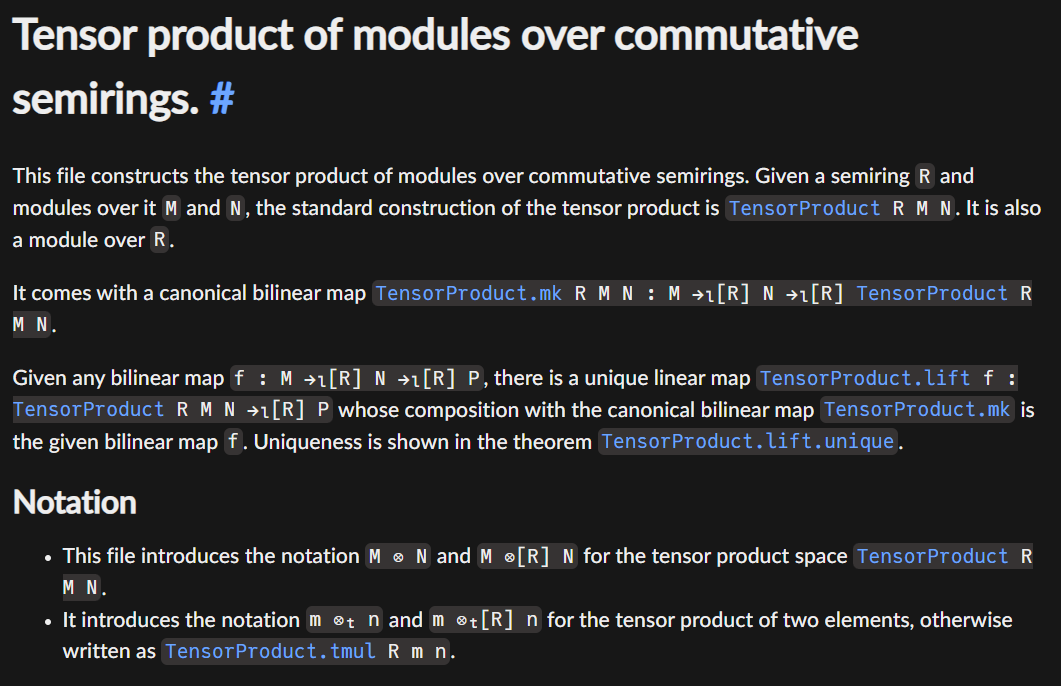
\includegraphics[width=1\linewidth]{image2.png}

\end{frame}
\begin{frame}{Extension of quadratic forms by scalars in Mathlib}


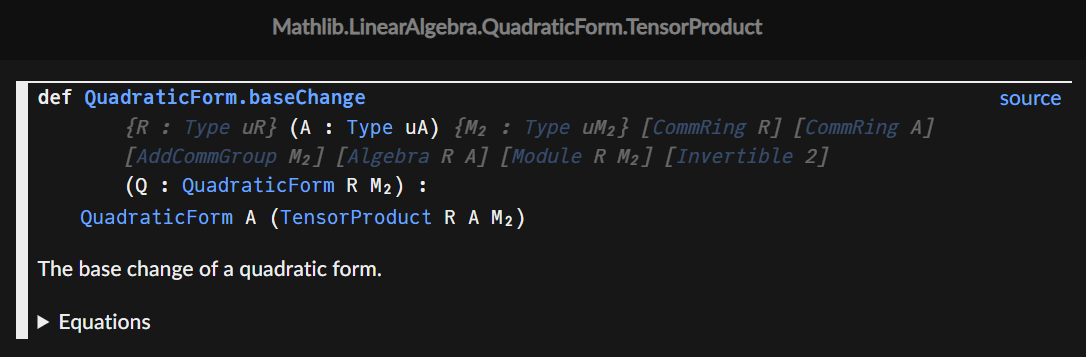
\includegraphics[width=1\linewidth]{image3.png}

\end{frame}
% Polynomial Module equivalence
\begin{frame}{Polynomial Module equivalence}

We can view $V[t]=F[t] \otimes_F V$ similarly to (formal) polynomials as sums $v_0+v_1X^1+v_2X^2+\dots$. \\

\pause This interpretation is implemented in Mathlib as \textbf{PolynomialModule $F$ $V$}, with data $\mathbb N \to_0 V$. \\

\pause 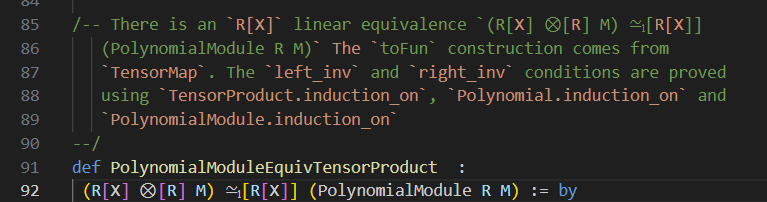
\includegraphics[width=1\linewidth]{image4.png}

\end{frame}
% Degree over polynomial module
\begin{frame}{Degree}

Degree is fairly easy to define over $\mathbb N \to_0 V$ as the 'maximum' or 'supremum' of the support. It would be much more difficult to define degree on $F[t] \otimes_F V$. 

\pause 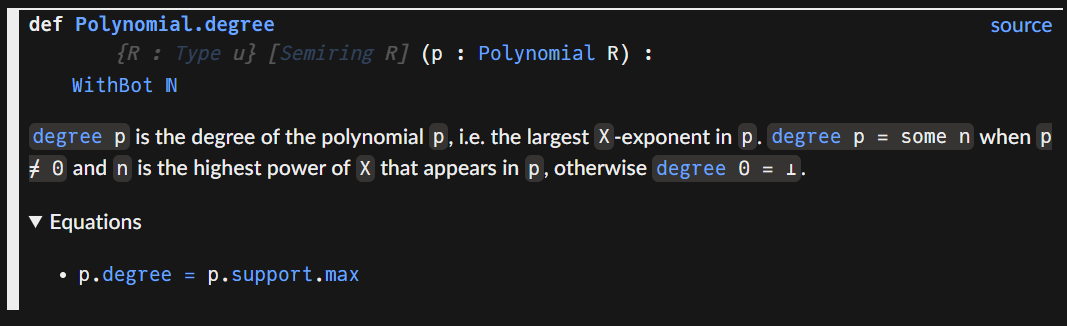
\includegraphics[width=1\linewidth]{image5.png}

\end{frame}
% Implicit conversions, the downard chain
\begin{frame}{The downward chain}
We have a map $(\mathbb N \to_0 V) \to F[t] \otimes_F V$ from the prior equivalence. We also have a natural map $F[t] \to F(t)$ (from Mathlib), which gives us a map $F[t] \otimes_F V \to F(t) \otimes_F V$. 

\centering

\pause 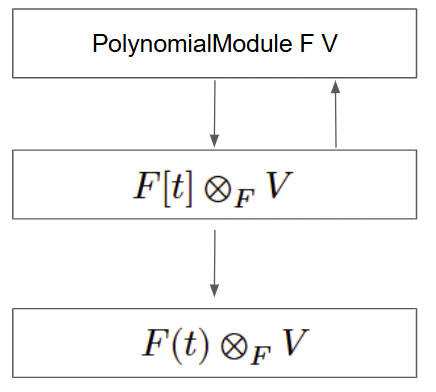
\includegraphics[width=0.5\linewidth]{image11.png}


\end{frame}

\begin{frame}{Implicit Conversions}



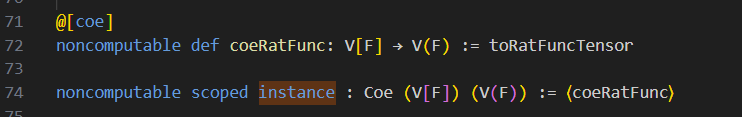
\includegraphics[width=1\linewidth]{image7.png}


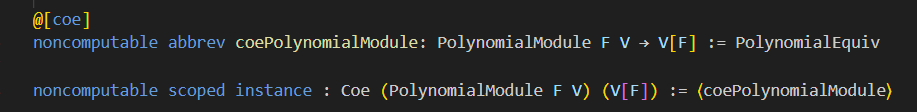
\includegraphics[width=1\linewidth]{image8.png}


\end{frame}


\begin{frame}{Notation}
\begin{figure}
    \centering
    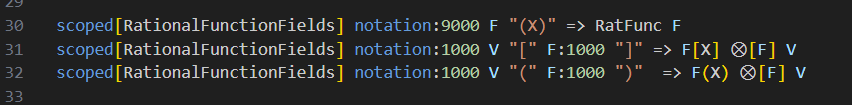
\includegraphics[width=1\linewidth]{image9.png}
\end{figure}
\end{frame}

\section{Conclusion}

\begin{frame}{References}
\begin{enumerate}
\item Conrad, K. (n.d.). Bilinear Forms. https://kconrad.math.uconn.edu/blurbs/linmultialg/bilinearform.pdf
\item Elman RS, Karpenko N, Merkurjev A. The Algebraic and Geometric Theory of Quadratic Forms. American Mathematical Society; 2008.
%\item 
%\item Avigad, J. Buzzard, K. Lewis R. Y. Massot, P. (2020). \textit{Mathematics in Lean}. 
%\item Liesen, J. Mehrmann, V. (2015). \textit{Linear Algebra}.
%\item Reich, E. (2005, February 28). Bilinear Forms. Retrieved July 10, 2005, from https://math.mit.edu/~dav/bilinearforms.pdf

\end{enumerate}
\end{frame}


\begin{frame}
	    \begin{center}
	        \textbf{Thank you!}\\
	        
	        Special thanks to Dr. George McNinch and the REU
         \bigbreak
         \LARGE
       
	    \end{center}
\end{frame}



\end{document} 